\chapter{FPGA的数字运算}
\begin{introduction}
  \item 有符号数、无符号数的四则运算\textit{Verilog}仿真
  \item \textit{N-bit} 系数量化下系统频率响应\textit{MATLAB}仿真
  \item 有限字长效应的\textit{MATLAB}仿真
\end{introduction}
\section{实验背景和目的}

在数字信号处理系统中,定点数表示和量化误差是非常关键的问题,尤其在进行信号运算和滤波器设计时。随着数字系统的普及,定点数逐渐成为实现高效计算的重要工具。定点数的有限字长效应可能导致数值精度损失,进而影响系统的性能和输出结果。因此,研究定点数在数字运算中的应用,尤其是在滤波器系数量化过程中的影响,具有重要的理论和实践意义。

本实验的目的在于深入探讨数字运算中的定点数表示,研究不同量化方式(如截断与舍入)对系统频率响应的影响,以及有限字长效应如何在实际应用中造成量化误差。通过对定点数和量化误差的理论分析与实验验证,进一步加深对数字信号处理系统的理解,提升对量化与误差控制技术的实际应用能力。

通过本实验,学生将掌握定点数运算的基本原理,理解量化过程中的误差产生机制,并能够在不同量化位宽下评估系统性能。同时,实验也为后续的滤波器设计与系统优化提供了基础,帮助学生更好地应对数字信号处理中常见的精度限制问题。
\section{实验原理}
\subsection{数字运算中使用的定点数}
一般而言,为了硬件存储的方便,数字运算中采用定点数进行运算。尤其是在通信系统中,大多采用不超过16比特的二进制定点数进行数据的存储。\footnote{浮点数也是常用的存储方式,但和本实验关联不大,故不具体叙述。}
在定点数表示中,常见的符号表示方法包括原码、补码和反码。

\textbf{原码}是一种最直观的符号数表示方法,最高位用于表示符号,剩余位数表示数值的绝对值。当符号位为0时,表示正数;当符号位为1时,表示负数。例如,假设采用8比特表示整数:
\[
+5 \Rightarrow 00000101
\]
\[
-5 \Rightarrow 10000101
\]
原码的主要缺点是存在两个零的表示,即 \(+0 = 00000000\) 和 \(-0 = 10000000\),这在运算过程中会导致额外的复杂性。


\textbf{反码}的表示方法是:正数的表示与原码相同,而负数的表示方式是对其对应的正数按位取反(即0变1,1变0)。例如:
\[
+5 \Rightarrow 00000101
\]
\[
-5 \Rightarrow 11111010
\]
反码的优点是加法运算可以直接进行,但仍然存在两个零的表示,即 \(+0 = 00000000\) 和 \(-0 = 11111111\)。


上面两种表示方式各有缺点,因此\textbf{补码}是计算机系统中最常用的定点数表示方法。正数的表示与原码相同,而负数的补码表示是对其对应正数的反码加1。例如:
\[
+5 \Rightarrow 00000101
\]
\[
-5 \Rightarrow 11111011
\]
补码的最大优点在于加法运算可以直接进行,无需额外的进位处理,同时消除了反码中的双零问题,使得只有 \(00000000\) 表示零。此外,补码还能使符号位与数值部分一起参与运算,从而简化了电路实现。

在通信系统、信号处理以及硬件实现中,补码由于其高效性和简化运算的特性,被广泛应用于定点数运算。
\subsection{系数量化造成有限字长效应}
一般而言,为了硬件存储的方便,数字信号处理器(DSP)中通常采用有限精度的定点数进行运算。然而,由于有限精度表示,滤波器系数在量化后会引入误差,这种误差对系统性能的影响称为系数量化效应。

在实际DSP实现中,滤波器的系数也需要用有限比特宽度的定点数或浮点数进行表示。当理想滤波器系数 \( h[n] \) 量化为有限比特宽度的表示 \( \hat{h}[n] \) 时,会引入量化误差:
\begin{equation}
e[n] = h[n] - \hat{h}[n]
\end{equation}
这种误差会导致滤波器的幅频响应和相频响应偏离理想情况,并可能引入额外的增益或相位畸变。


对于无限脉冲响应(IIR)滤波器,系数量化误差可能导致极点的位置发生偏移,进而影响系统的稳定性。当极点位于单位圆外时,滤波器就会不稳定。因此,在IIR滤波器设计中,需要特别关注系数量化对极点分布的影响,并可采用高精度系数或级联结构来减小量化误差的影响。


对于有限脉冲响应(FIR)滤波器,系数量化主要影响滤波器的频率响应,导致幅频特性偏差。然而,由于FIR滤波器没有极点,因此量化不会影响系统的稳定性。为了减小量化误差,可以采用较高比特宽度的系数表示,或者利用最佳逼近方法来优化量化方案。

为了减小系数量化效应,通常采用以下几种方法:
\begin{itemize}
    \item \textbf{增加比特宽度}:提高系数的表示精度,以降低量化误差。
    \item \textbf{采用级联结构}:在IIR滤波器中,使用级联二阶节(biquad structure)可以减小极点的偏移,提高系统稳定性。
    \item \textbf{最小化量化误差}:采用最佳逼近方法,如均方误差(MSE)优化或其他优化算法,使量化误差最小化。
    \item \textbf{过采样}:通过提高采样率,使量化噪声的影响分布在更宽的频带范围内,然后利用抗锯齿滤波减少有害影响。
\end{itemize}

在DSP系统设计中,系数量化效应是不可避免的,但通过合理的设计策略,可以有效降低其对系统性能的影响。
\subsection{A/D量化器中产生的量化噪声}
在数字信号处理中,模拟信号需要经过模数转换(A/D转换)才能在数字系统中进行处理。然而,由于A/D转换器的有限分辨率,输入信号在量化过程中会产生量化误差,这种误差表现为量化噪声,并影响信号质量。为了衡量量化噪声对信号的影响,通常采用量化信噪比(SQNR, Signal-to-Quantization-Noise Ratio)来评估系统性能。


在A/D转换过程中,模拟信号 \( x(t) \) 经过取样后得到离散信号 \( x[n] \),然后被映射到有限比特数的数字表示 \( \hat{x}[n] \),通常假设产生的量化误差分布均匀且在\([- \Delta /2, \Delta /2]\) 之间,其中 \( \Delta \) 为量化步长。若信号的量化误差服从均匀分布,则可以计算其均方误差(即量化噪声的功率):
\begin{equation}
  \sigma_q^2 = \frac{\Delta^2}{12}
\end{equation}


其中,量化步长 \( \Delta \) 由ADC的分辨率 \( B \) 和满量程范围 \( V_{\max} - V_{\min} \) 确定:
\begin{equation}
  \Delta = \frac{V_{\max} - V_{\min}}{2^B}
\end{equation}


\textbf{量化信噪比}(SQNR,Signal-to-Quantization-Noise Ratio)定义为信号的均方值与量化噪声功率的比值,通常采用分贝(dB)表示:
\[
\text{SQNR} = 10 \log_{10} \left( \frac{\sigma_x^2}{\sigma_q^2} \right)
\]
假设输入信号为均匀分布或满幅正弦波,其均方值可表示为:
\[
\sigma_x^2 = \frac{(V_{\max} - V_{\min})^2}{12}
\]
代入量化噪声功率 \(\sigma_q^2\) 后,可以得到SQNR的表达式:
\[
\text{SQNR} = 6.02B + 1.76 \quad \text{(dB)}
\]
从该公式可以看出,A/D转换器的分辨率 \( B \) 每增加1比特,SQNR约提升 6.02 dB。

为了减小量化噪声,提高系统的量化信噪比,可以采用以下几种方法:
\begin{itemize}
    \item \textbf{增加ADC的位数}:提高量化分辨率 \( B \),从而减小量化误差,提高SQNR。
    \item \textbf{增大输入信号幅度}:适当调整输入信号的动态范围,使其接近ADC的满量程范围,从而充分利用量化级数,提高信号能量。
    \item \textbf{过采样}:通过提高采样率,将量化噪声的频谱展宽,然后利用抗锯齿滤波减少有害噪声,等效提高SQNR。
    \item \textbf{采用噪声整形技术}:在高阶A/D转换器(如Sigma-Delta ADC)中,利用反馈结构将量化噪声移出信号带宽,提高信号质量。
\end{itemize}

在数字信号处理和通信系统中,量化噪声是不可避免的,但通过优化ADC设计和信号处理策略,可以有效降低其影响,提高系统性能。在本次实验中,我们重点讨论 N-bit 系数量化下系统频率响应以及运算有限字长效应对滤波器输出响应的影响。

\section{实验使用软件}
\begin{itemize}
  \item Visual Studio Code,用于Verilog 文件的撰写;
  \item iverilog,用于Verilog编译;
  \item gtkwave,用于波形显示。
  \item MATLAB R2024b,用于系数量化和有限字长效应实验。
\end{itemize}
\section{实验内容}
\subsection{有符号数、无符号数的四则运算Verilog仿真}
在数字电路设计中,处理有符号数与无符号数的运算是基础且关键的任务。由于计算机通常采用补码表示有符号数,因此在进行加、减、乘、除等四则运算时,必须特别注意符号扩展和进位处理。本实验通过 Verilog 编写四则运算模块,分别实现有符号数和无符号数的计算,并通过仿真验证其正确性。
\subsubsection{模块外部接口定义}
为了模块更利于用户理解,四则运算使用相同名称的I/O接口,列举如表~\ref{table:interface}~。
\begin{table}[htbp]
    \centering
    \begin{tabular}{ccc}
      \toprule
       信号名 & 意义 & 端口类型\\
      \midrule
        \texttt{i\_a} & 运算模块的第一个输入 & Input \\
       \texttt{i\_b} & 运算模块的第二个输入 & Input \\
       \texttt{signed\_result} & 有符号数输出 & Output \\
       \texttt{unsigned\_result} & 无符号数输出 & Output \\
      \bottomrule
    \end{tabular}
    \caption{运算模块接口说明}
    \label{table:interface}
\end{table}
\subsubsection{模块功能说明}
以\textbf{ADD}模块为例,说明模块的功能。ADD模块的代码如下所示。
\begin{lstlisting}[language=verilog]
  module ADD(
    input [3:0] i_a,
    input [3:0] i_b,
    output [4:0] o_unsigned_result,
    output [4:0] o_signed_result
);

wire signed [3:0] signed_a;
wire signed [3:0] signed_b;

assign signed_a = i_a;
assign signed_b = i_b;
assign o_unsigned_result = i_a + i_b;
assign o_signed_result = signed_a + signed_b;

endmodule
\end{lstlisting}

如代码所示,它实现了位宽为4的信号\texttt{i\_a}和\texttt{i\_b}作为无符号数或有符号数的相加,结果预留一位作为最高位进位的存储。其它三种运算类似\texttt{ADD}模块的写法,此处不再赘述。
\subsubsection{模块测试}
以\textbf{ADD}模块的测试为例,其余三个模块类似该模块的测试。将所有输入可能性写入Test case,编写 Verilog Testbench如下:
\begin{lstlisting}{language=verilog}
  `timescale 1ns/1ps

module tb_ADD;

    reg [3:0] a;
    reg [3:0] b;
    wire [4:0] signed_result;
    wire [4:0] unsigned_result;

    ADD dut(
        .i_a(a),
        .i_b(b),
        .o_signed_result(signed_result),
        .o_unsigned_result(unsigned_result)
    );
    integer i, j;

    initial begin
        a = 4'd0; b = 4'd0; #10;
        a = 4'd0; b = 4'd1; #10;
        a = 4'd0; b = 4'd2; #10;
        // ...
        a = 4'd0; b = 4'd14; #10;
        a = 4'd0; b = 4'd15; #10;
        // ...

        a = 4'd15; b = 4'd10; #10;
        a = 4'd15; b = 4'd11; #10;
        a = 4'd15; b = 4'd12; #10;
        a = 4'd15; b = 4'd13; #10;
        a = 4'd15; b = 4'd14; #10;
        a = 4'd15; b = 4'd15; #10;
    #1000 $finish;
    end

    initial begin
        $dumpfile("add.vcd");
        $dumpvars(0,tb_ADD);
    end
endmodule
\end{lstlisting}
用iverilog编译器编译待测模块和Testbench,得到仿真波形文件(vcd格式),之后使用轻量级波形预览软件GTKwave进行波形预览,得到四则运算的测试波形图如图~\ref{fig:verilog_test}~。\footnote{为了符合四则运算的直观认识,对于有符号数部分的输入输出,采用了\texttt{signed\_decimal}格式,而对无符号数部分采用了\texttt{decimal}格式。}
\begin{figure}[htbp]
  \centering
  \subfloat[\texttt{ADD}模块部分测试数据]{\includegraphics[width=0.95\textwidth]{figure/exp2/wave_add.png}}
  \newline
  \subfloat[\texttt{SUB}模块部分测试数据]{\includegraphics[width=0.95\textwidth]{figure/exp2/wave_sub.png}}
  \newline
  \subfloat[\texttt{MUL}模块部分测试数据]{\includegraphics[width=0.95\textwidth]{figure/exp2/wave_mul.png}}
  \newline
  \subfloat[\texttt{DIV}模块部分测试数据]{\includegraphics[width=0.95\textwidth]{figure/exp2/wave_div.png}}
  \caption{有符号数、无符号数四则运算Verilog仿真的部分测试数据}
  \label{fig:verilog_test}
\end{figure}

可以看到,对于加、减、乘三种运算,仿真结果均显示了正确的结果,没有溢出现象的发生。对于除运算,输出结果为向下取整。当除数为0时,输出结果为“X”(即不确定),这也符合预期。  

\subsection{N-bit 滤波器系数量化下系统频率响应MATLAB仿真}
构建一个IIR滤波器,其系统函数为:
\begin{equation}
  H(z) = \frac{0.05}{1+1.7z^{-1}+0.745z^{-2}}
\end{equation}
教材中已给出8-bit系数量化效应下系统单位脉冲频率响应与无限精度的系统频率响应的对比。结果表明:有限精度下系统的频率响应幅度会下降。为了进一步探究这种频率响应的变化原因,更改量化位宽后重新进行仿真。选择量化位宽为10-bit,6-bit,4-bit,量化方式为\texttt{round}(四舍五入),将单位脉冲序列为输入时的频率响应与原系统频率响应进行比较。编写MATLAB代码如下。


\begin{lstlisting}{language=matlab}
b = 0.05;
a = [1, 1.7, 0.745];

% 归一化
max_a_b = max(max(b), max(a));
b1 = b / max_a_b;
a1 = a / max_a_b;

% 量化位数
Q = [10, 6, 4];

% 计算量化系数
scale_factors = 2.^(Q - 1) - 1;
b_quant = round(b1 * scale_factors);
a_quant = round(a1' * scale_factors); 

% 生成脉冲输入
N = 2048;
xn = (0:N-1) / N * 2;
dn = [1, zeros(1, N-1)];

% 计算原系统的频率响应
hn = filter(b, a, dn);
fn = 10 * log10(abs(fft(hn, N)));
fn = fn - max(fn); % 归一化

% 绘制原系统的频率响应
figure;

plot(xn(1:N/2), fn(1:N/2), '-k', 'LineWidth', 1.5);
hold on;
legend_entries = ["原系统的频率响应"];

% 计算量化后的频率响应
for i = 1:length(Q)
    hn_quant = filter(b_quant(i), a_quant(:,i)', dn);
    fn_quant = 10 * log10(abs(fft(hn_quant, N)));
    fn_quant = fn_quant - max(fn_quant);
    % 绘制量化后的频率响应
    plot(xn(1:N/2), fn_quant(1:N/2), '--', 'LineWidth', 1.2);
    legend_entries = [legend_entries, sprintf('%d 比特量化后的频率响应', Q(i))];
    
    % 计算并输出量化系统的极点
    s_quant = roots(a_quant(:,i));
    disp(['量化位数 ', num2str(Q(i)), ' 的极点:']);
    disp(s_quant);
end

% 设置图例和坐标轴标签
xlabel('归一化频率(f_s/2)',"Interpreter","tex");
ylabel('归一化幅度(dB)');
legend(legend_entries, 'Location', 'Best');
title("原系统、10比特、6比特、4比特量化位宽量化频率响应");
grid on;
hold off;

\end{lstlisting}

运行该代码,得到舍入方式下的频率响应如图~\ref{fig:RND}~。将该代码中的\texttt{round}替换为\texttt{floor}就可以得到截断方式的仿真结果,如图~\ref{fig:TRN}~所示。
\begin{figure}[htbp]
  \centering
  \subfloat[舍入方式\label{fig:RND}]{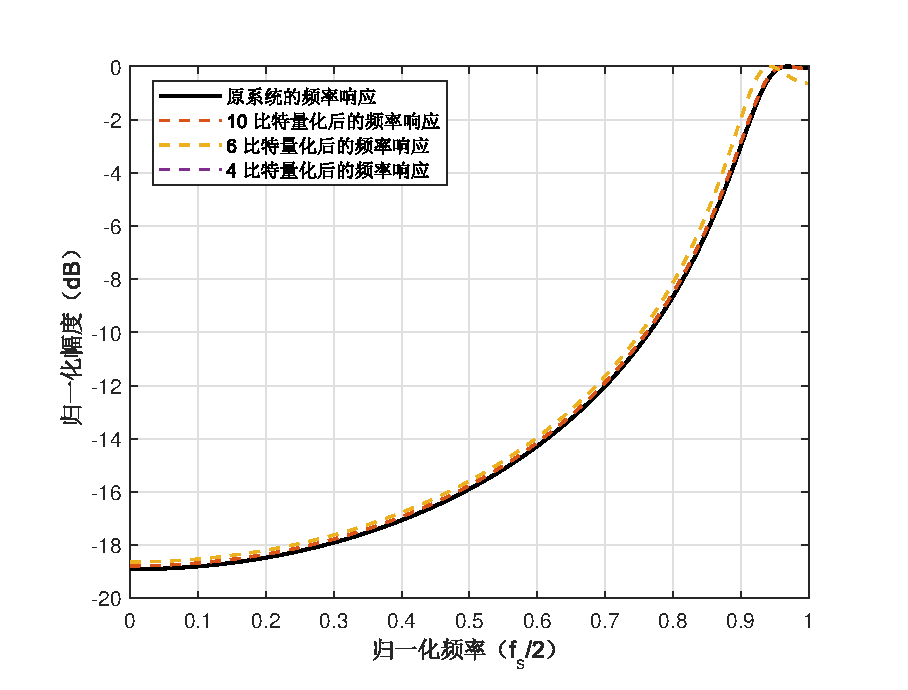
\includegraphics[width=0.45\textwidth]{figure/exp2/2-2round.eps}}
  \hfill
  \subfloat[截断方式\label{fig:TRN}]{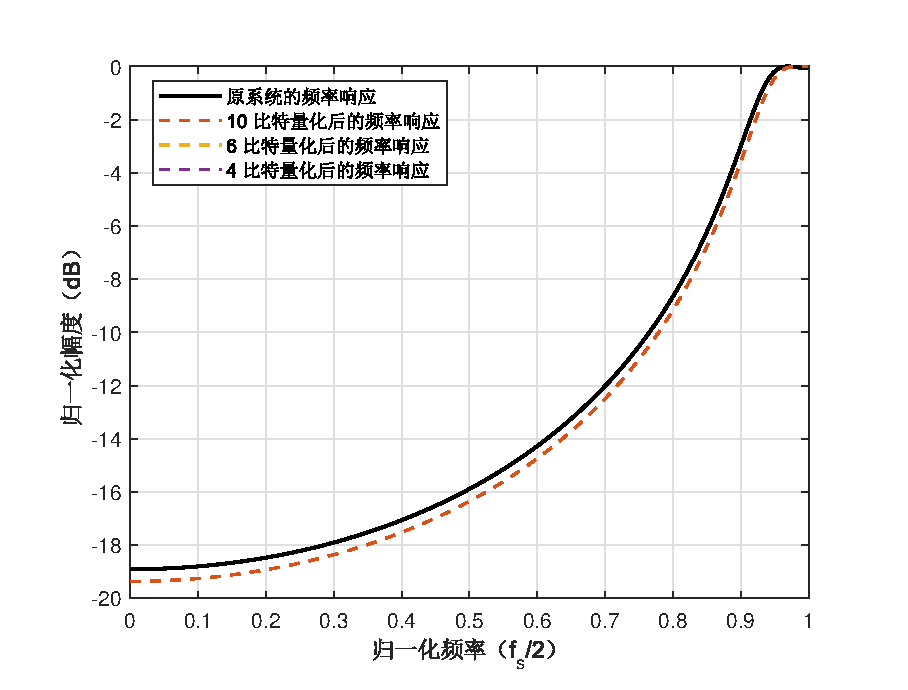
\includegraphics[width = 0.45\textwidth]{figure/exp2/2-2truncate.eps}}
  \caption{原系统,10-bit,6-bit,4-bit系数截断/舍入量化下的系统频率响应}
\end{figure}

可以看到,截断方式下4-bit和6-bit的仿真图线和舍入方式下的4-bit仿真图线都没有正常显示,经过检查发现:此时滤波器的分子系数被量化为0,导致输出响应为0。此时系统的极点也为纯实数。另外,舍入方式下,系统的频率响应随着量化位数的增加而有些许降低;截断方式下,系统的频率响应随着量化位数的增加而有些许上升。这可能是因为舍入方式下系数量化引入了小幅误差,误差随位宽增加逐渐减少,使系统频率响应整体趋向下降。而截断方式下始终往 0 方向偏移,使得系统初始增益降低,随着位宽增加,增益逐渐恢复,导致频率响应上升。\footnote{并不确定这种表述的正确性。}并且,截断方式下,相同量化位数引入的误差大于舍入方式下引入的误差。这是因为舍入方式下系数会朝着更贴近真实系数的方向量化,而截断方式下系数永远会向下量化,从而有更大的可能性获得更大的误差。\footnote{将分子系数换为0.5时,四种仿真图线全能够正常显示,这是因为此时滤波器系数的分子会被量化为一个整数而不是0,使得单位脉冲响应作用下的系统频率响应存在。因此可以将滤波器系数同乘一个常数,或提升单位脉冲响应的幅值。}


\subsection{运算有限字长效应的MATLAB仿真}
在系数量化效应的实验中,我们在滤波器系数创建时就将其使用截断或舍入方式量化。而在运算有限字长效应的实验中,我们默认滤波器系数是理想的,并在输出部分加一次舍入量化。令输入$x[n] = \frac{7}{8}\delta(n)$,观察2-bit,4-bit,6-bit量化效应下的输出响应。编写MATLAB代码如下:
\begin{lstlisting}[language=matlab]
clc; clear; close all;

% Input
x = [7/8 zeros(1, 15)];
N = length(x);
y = zeros(1, N);
% Coefficients
A = 0.5;
B_values = [2, 4, 6]; % Data Width
Qy_results = cell(1, length(B_values)); % Storage Init

% Original
for i = 1:N
    if i == 1
        y(i) = x(i);
    else
        y(i) = -A * y(i-1) + x(i);
    end
end
% 需要注意的是,系统在每一次计算出结果时,都会进行一次输出结果量化,因此不能用filter函数进行计算
% Quantized
for b_idx = 1:length(B_values)
    B = B_values(b_idx);
    Qy = zeros(1, N); % 初始化存放量化结果

    for i = 1:N
        if i == 1
            Qy(i) = x(i);
        else
            Qy(i) = -A * Qy(i-1) + x(i);
        end
        % RND
        Qy(i) = round(Qy(i) * (2^(B-1))) / 2^(B-1);
    end
    
    Qy_results{b_idx} = Qy;
end
colors = [0, 0.447, 0.741;  % 亮蓝色
          0.850, 0.325, 0.098;  % 鲜橙色
          0.494, 0.184, 0.556;  % 深紫色
          0.466, 0.674, 0.188]; % 鲜绿色

markers = {'o', 's', 'd', '^'}; % 圆点, 方块, 菱形, 三角形
xa = 0:N-1;
figure; hold on;

plot(xa, y, '-o', 'Color', colors(1, :), 'MarkerFaceColor', colors(1, :), ...
    'LineWidth', 1, 'MarkerSize', 6, 'DisplayName', '原系统运算结果');

for b_idx = 1:length(B_values)
    B = B_values(b_idx);
    Qy = Qy_results{b_idx};
    plot(xa, Qy, '-o', 'Color', colors(b_idx + 1, :), 'MarkerFaceColor', colors(b_idx + 1, :), ...
        'LineWidth', 1, 'Marker', markers{b_idx + 1}, 'MarkerSize', 6, ...
        'DisplayName', sprintf('%d-bit 量化结果', B));
end

legend;
xlabel('运算次数');
ylabel('滤波结果');
grid on;

xlim([-1, N]); % X 轴范围
y_min = min([y, Qy_results{:}]) - 0.1; % 计算所有数据的最小值
y_max = max([y, Qy_results{:}]) + 0.1; % 计算所有数据的最大值
ylim([y_min, y_max]); % 设置 Y 轴范围
\end{lstlisting}

运行该代码,得到原系统与三种量化位宽进行输出结果量化后的结果随运算次数(序列长度)的变化如图~\ref{fig:2-3}~。可以看到,随着运算次数增加,量化后的三条曲线均出现了在两个量化电平间不断切换的现象。

\begin{figure}[htbp]
  \centering
  \begin{minipage}{0.5\linewidth}
    \baselineskip = 1.25 \baselineskip
    一般而言,量化误差的误差来源为以下三种:
    \begin{itemize}
        \item \textbf{舍入误差(Rounding Error)}:由于量化过程中数值需要映射到有限比特位表示的离散值,导致计算结果与理论值之间存在误差。
        \item \textbf{极限环振荡(Limit Cycle Oscillation)}:在反馈系统或 IIR 滤波器中,有限精度计算可能导致信号在若干固定值之间振荡,而无法进一步衰减。
        \item \textbf{量化噪声(Quantization Noise)}:低比特位量化会引入类似噪声的现象,使信号无法平滑下降到零,而是在某个范围内不规则波动。
    \end{itemize}

    通过对比实验数据,我们观察到以下现象:

    \begin{itemize}
        \item 在\textbf{无限精度计算}条件下,信号能平滑衰减至零,符合理论期望。
        \item 在\textbf{有限精度计算}条件下,当信号幅值降低到一定范围时,输出值在某些固定值处振荡,无法继续趋近于零。
        \item \textbf{量化比特位越低},信号的跳变幅度越大,震荡现象越明显。
    \end{itemize}


  \end{minipage}
  \hfill
  \begin{minipage}{0.45\linewidth}
    \centering
    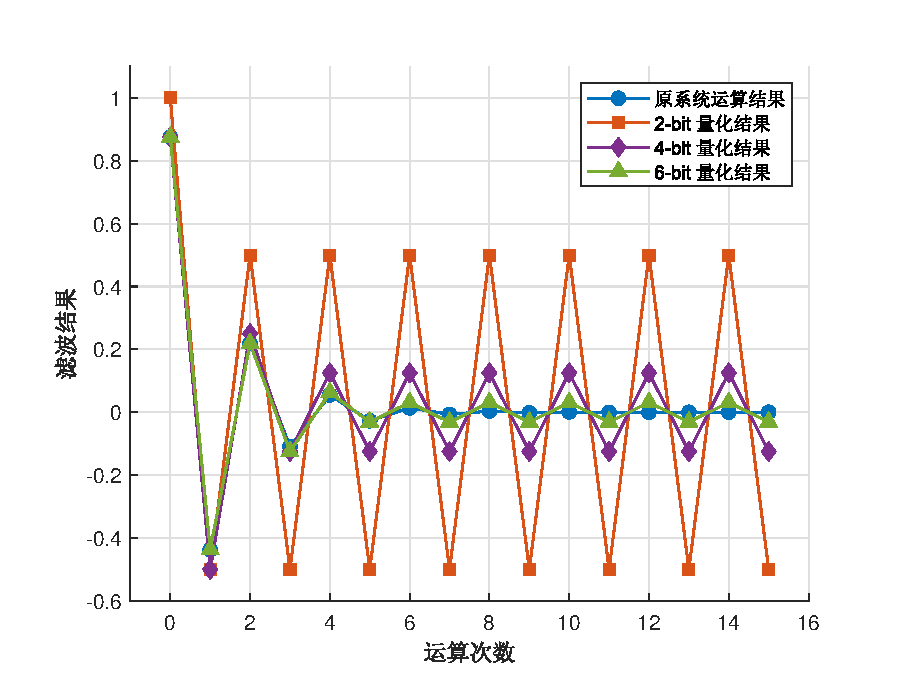
\includegraphics[width=0.95\linewidth]{figure/exp2/2-3.eps}
    \caption{原系统,2-bit,4-bit,6-bit运算量化下输出结果的对比}
    \label{fig:2-3}
  \end{minipage}
\end{figure}

根据本实验的实验结果,推测出现图~\ref{fig:2-3}~中的波形的原因是极限环振荡。

